\documentclass{article}

\usepackage{fontspec}
\usepackage{mathptm}
\usepackage{comment}
\usepackage{booktabs}
\usepackage{amsmath}
\usepackage{geometry}
\usepackage{graphicx}
\usepackage{microtype}
\usepackage{hyperref}
\usepackage{fancyvrb}
\usepackage{float}


\defaultfontfeatures{Mapping=tex-text}
\setmainfont{Times}
%\setmonofont{Consolas}
\setmonofont{Inconsolata}

\title{Ceph Parallel File System Evaluation Report}
\author{Feiyi Wang, Sarp Oral, Doug Fuller, Blake Caldwell, James Simmons\\
Brad Settlemyer, Scotty Atchley, Jason Hill, Mark Nelson}

%% adjust float figure placement
\renewcommand{\textfraction}{0.15}
\renewcommand{\topfraction}{1.00}
\renewcommand{\bottomfraction}{0.70}
\renewcommand{\floatpagefraction}{0.85}

\begin{document}

\maketitle
%\authorrunning{}
%\titlerunning{}

\section{Introduction}

NCCS contracted Inktank, the major developer behind the open-sourced parallel
file system, Ceph, for a deep-dive study. It covers a wide range of technical
topics, ranging from system setup, deployment, administration to internal
mechanism. As part of this effort, we have set up a Ceph testbed within NCCS
for performance evaluation. The goal is to examine the suitability of Ceph
system as a potential candidate for our next-generation HPC storage solution.
This report presents our experience, results, and observations.

\section{Evaluation Environment Description}

The backend storage we use for this evaluation is DDN's SFA10K. It consists of
200 SAS drives and 280 SATA drives, driven by 4 hosts. Each host has
2 IB QDR connections to the storage backend. We configure and use 4 IB as
primary connections, which can saturate the maximum theoretical throughput,
around 11 - 12 GB/s. The connection diagram is illustrated as the following:

\begin{figure}[htb]
\centering
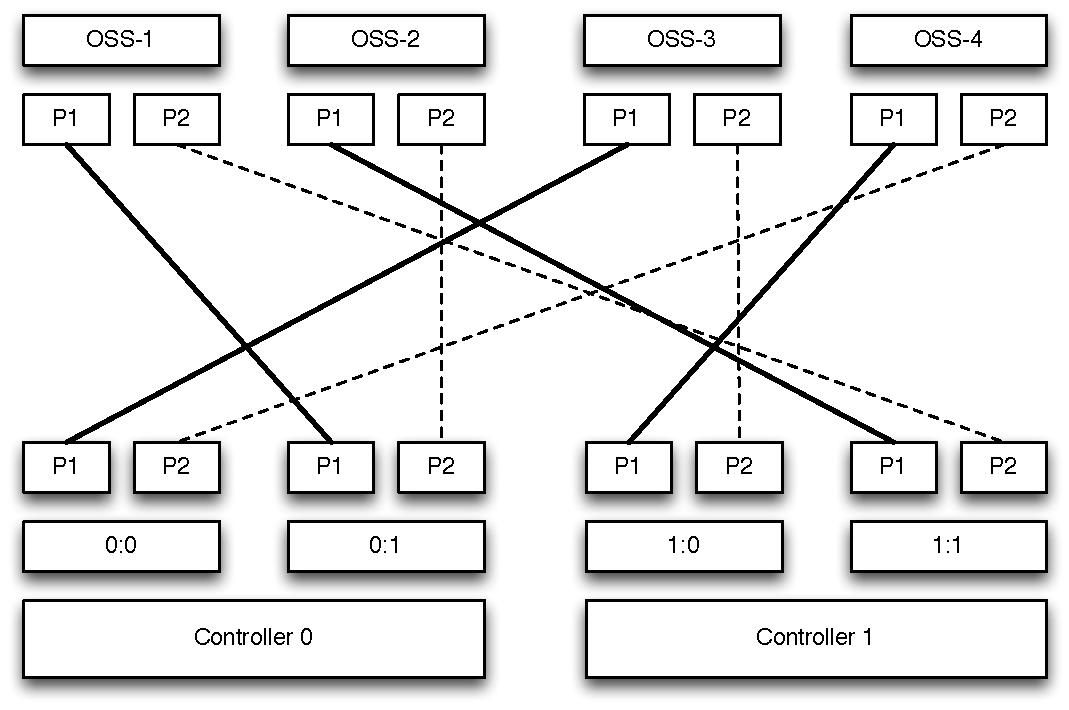
\includegraphics[width=4in]{figs/sfa10k}
\caption{DDN SFA10K Hardware Diagram}
\end{figure}


The supporting infrastructure nodes are summarized in the following table:

\begin{table}[htb]
\centering
    \begin{tabular}{ll}
    \toprule
    Node & Role \\
    \midrule
    tick-mds1 & Ceph monitor node \\
    spoon46 & Ceph MDS node \\
    tick-oss[1-4] & Ceph OSD servers \\
    spoon28-31, spoon37-41 & Ceph client nodes \\
    \bottomrule

    \end{tabular}

\end{table}

The hosts are running Redhat 6.3 with 3.5.1 kernel (rhl-ceph image), Glibc 2.12
with syncfs support, locally patched. The Ceph version is 0.55 release. For a
complete a list of hosts that are running ceph images, you can do:

\begin{Verbatim}
grep "rhel6-ceph" /etc/gedi/MAC.info
\end{Verbatim}


\section{Baseline Performance}

Before we dive into specific Ceph performance measurement, we need to establish
the baseline performance. At the block level, assuming each LUN is RAID6 8+2,
we have the following results:

\begin{table}[htb]
\centering
\begin{tabular}{ll}
    \toprule
    SAS single LUN sequential read & ~1.4 GB/s \\
    SATA single LUN sequential read & ~955 MB/s \\
    Single host with 4 SAS LUNs & ~ 2.8 GB/s \\
    Single host with 7 SATA LUNs & ~ 2.6 GB/s \\
    \bottomrule
\end{tabular}

\end{table}

Single host refers to one of tick-oss node. Overall, the entire SSU
performance has been measured to perform at 11GB/s, compare to advertised
12GB/s. Also note that we performed IP over IB test as Ceph doesn't have
native IB support. The single host performance is about 2.7 GB per second.
Later, we will see RADOS is performing a maximum of 5 to 6 GB per seconds with
4 hosts.  So, this test shows that we have enough network bandwidth.


\section{Ceph Evaluation}

In this section, we will discuss the setup and results of a series of Ceph
specific benchmark results.

\subsection{System Tuning}

After experimentation, this is a set of tuning parameters we apply:


\begin{table}[htb]
\centering
\begin{tabular}{ll}
    \toprule
    \verb!nr_requests! & 2048 \\
    \verb!read_ahead_kb! & 4096 \\
    \verb!scheduler! & deadline \\
    \verb!/proc/sys/net/ipv4/tcp_moderate_rcvbuf! & 0 \\
    \bottomrule
\end{tabular}

\end{table}

The last tuning in the table is to disable TCP auto tuning. We have observed
this will make a notable improvement on Ceph read performance. 


\subsection{XFS Performance}

As we are going to make use of production ready XFS file system as the backend
local file system for Ceph, we want to see the level of performance of XFS on
SFA10K and acquire a set of sensible configuration parameters.
It is not meant to be exhaustive and full sweep of the performance
spectrum. Rather, we sample a selected set of parameters (block size, queue
depth, request size, sequential read and write), and this is the configurations
we selected: mount with \verb!nobarrier,noatim,inode64! options. The
\verb!inode64! option had a notable improvement on sequential write (around
20\%).

\begin{figure}[htb]
\centering
%% -- 1st figure
\begin{minipage}[t]{0.5\linewidth}
\centering
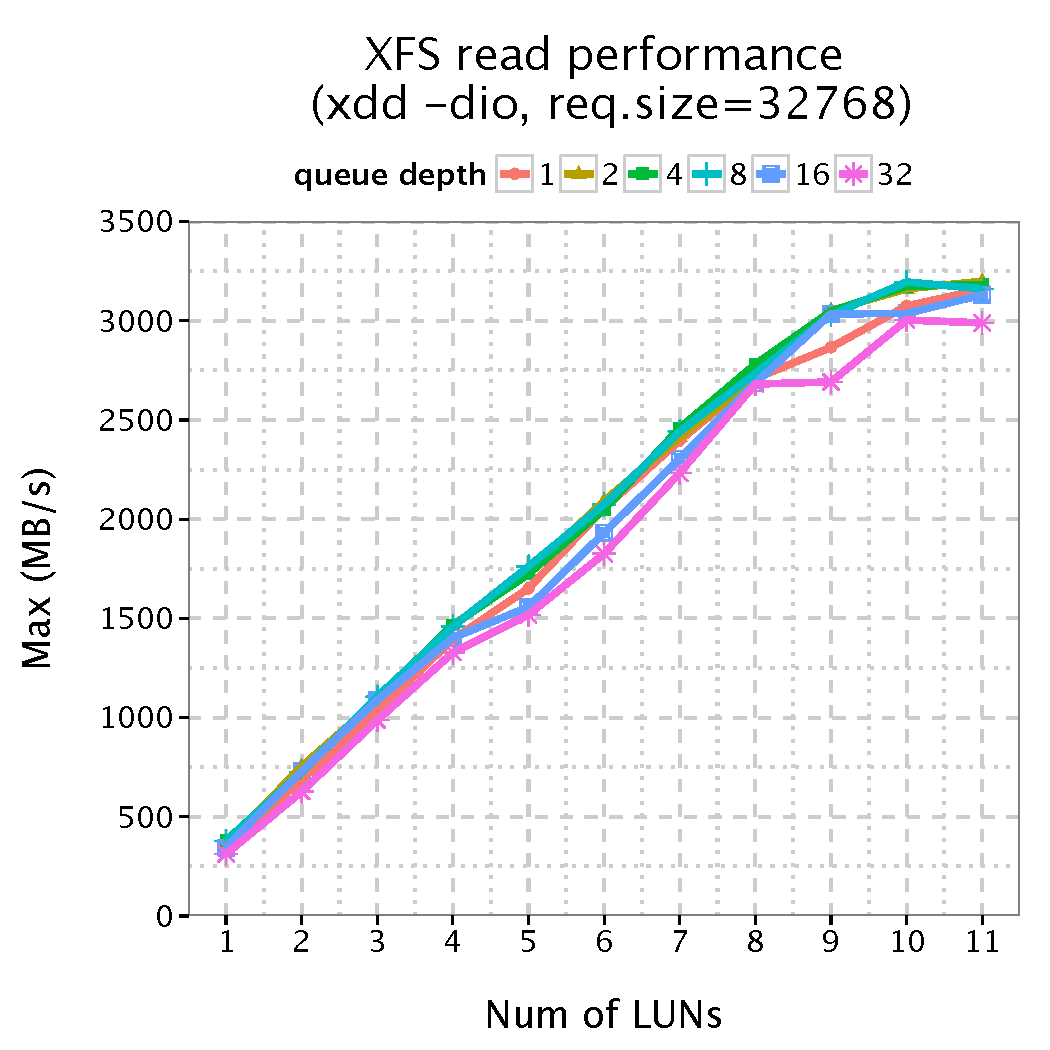
\includegraphics[width=3in]{data/xdd-read}
\caption{XFS read scaling on \# of devices}
\end{minipage}%
\begin{minipage}[t]{0.5\linewidth}
\centering
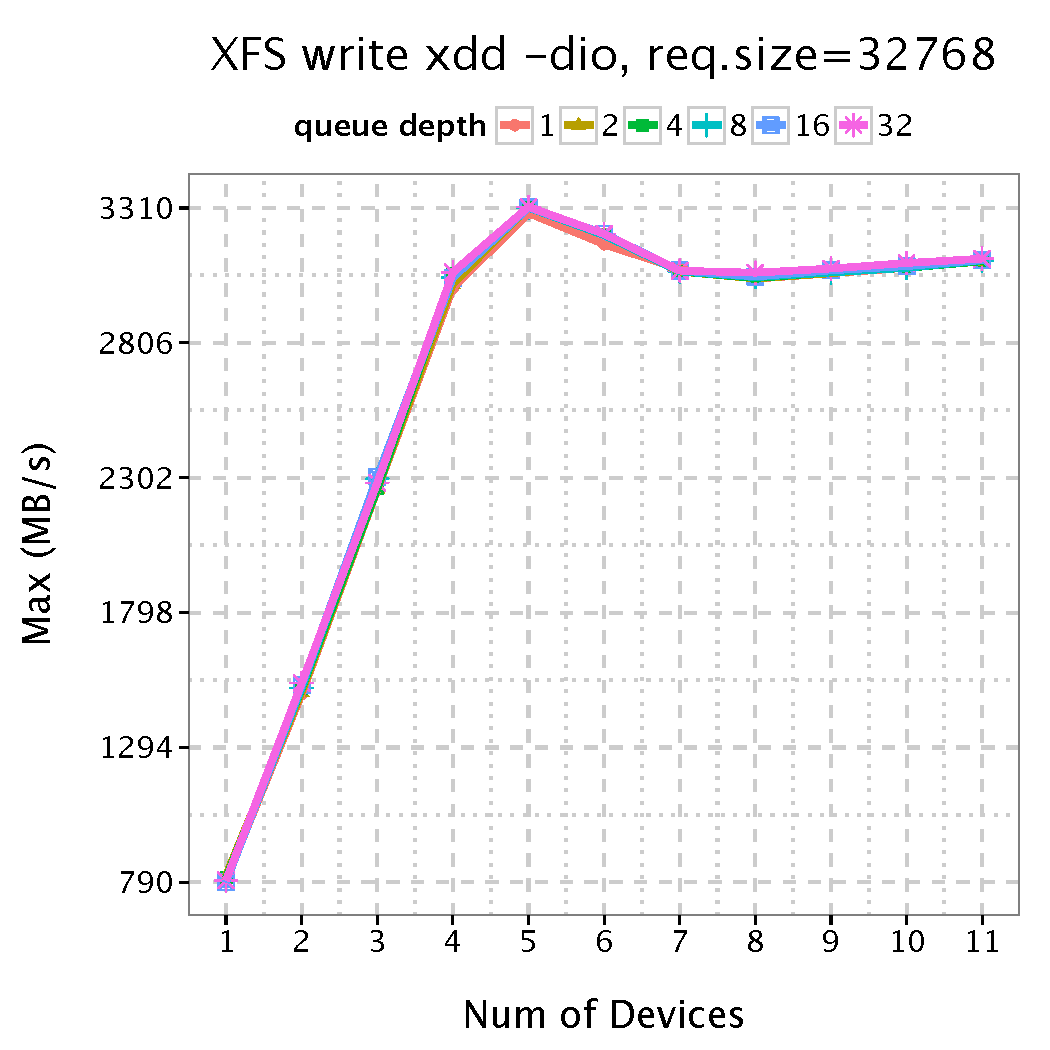
\includegraphics[width=3in]{data/xdd-write}
\caption{XFS write scaling on \# of devices}
\end{minipage}%
\end{figure}


The above scaling test on the number of devices indicates that XFS can get to
peak read performance with 5 SATA LUNs, then there is a bit of degradation from
there. The parameter space explored regarding to the queue depth doesn't seem
to make any obvious difference on performance though.


\subsection{Ceph RADOS Performance}

RADOS is Ceph object store, a foundational storage component for CephFS file
system. There are three types of scaling tests we are interested at RADOS layer:

\begin{itemize}
  \item scaling on the number of servers
  \item scaling on the number of clients
  \item scaling on the number of OSDs
\end{itemize}

Our system setup poses some limitation on the scalability test we want to
perform. In particular, we currently have 4 OSS server, 8 clients, and 11 OSD
per clients. So the scaling test will be within these constraints. However, we
can do larger scale test should the interest arise. 

\subsubsection{Scaling on number of OSDs}

In the following test, a single Ceph host drives $n$ number of OSDs. We
want to observe performance scaling properties when $n$ increases from 1 to
11. 

\begin{figure}[htb]
\centering
%% -- 1st figure
\begin{minipage}[t]{0.5\linewidth}
\centering
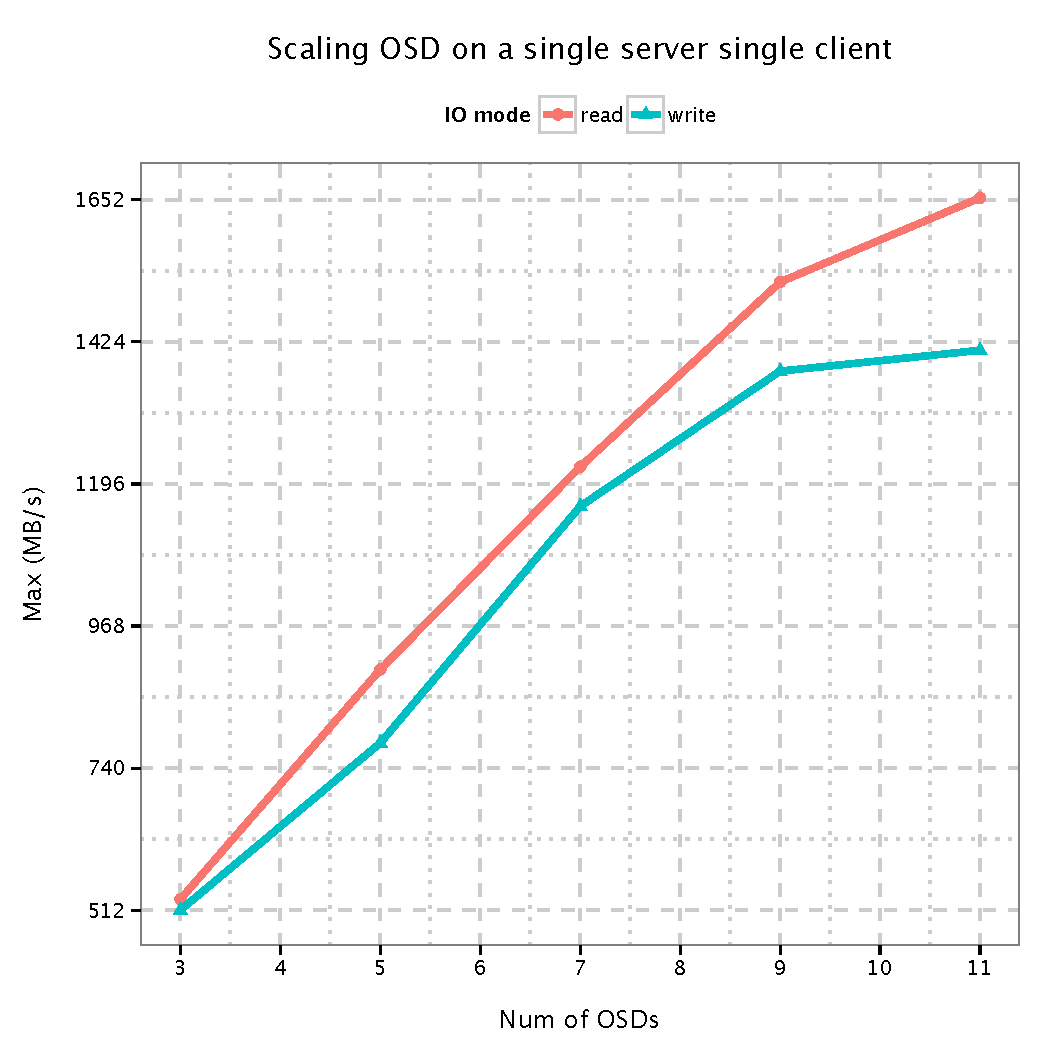
\includegraphics[width=3in]{data/rados_osd}
\caption{RADOS scaling on \# of OSDs}
\end{minipage}%
\begin{minipage}[t]{0.5\linewidth}
\centering
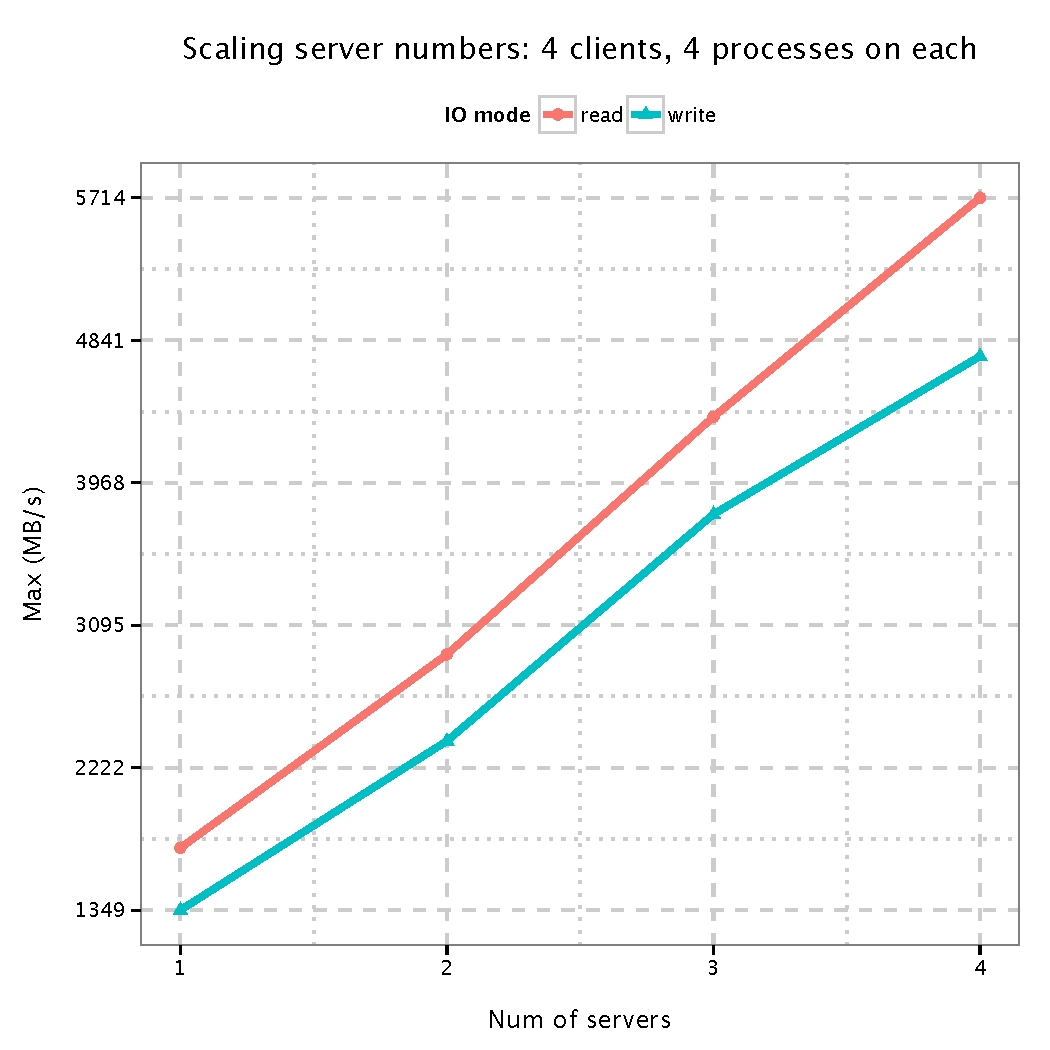
\includegraphics[width=3in]{data/rados_server}
\caption{RADOS scaling on \# of OSDs}
\end{minipage}%
\end{figure}

We observe that Ceph OSS exhibits near linear scalability up to 9 OSDs, and
still have room to grow at 11 OSDs. This suggests that we have not reached the
saturation point yet. The provisioning of more OSDs requires a SFA10K
reconfiguration, we will revisit this when time and resource permit.

\subsubsection{Scaling on number of servers}

In this test, we exercise OSS number from 1 to 4, driven by another 4 clients.
Each addition of OSS adds 11 more OSDs into the play. We observe that Ceph
exhibits linear scaling property with regard to number of servers as well, at
least in the given set of servers. However, the peak performance we are seeing
is about the half of what are expecting from SFA10K. The reasoning behind write
is attributed to the way Ceph perform journaling: Ceph doesn't support the
meta-data only journaling, therefore every write is equivalent of a
double-write: once to the data device, once to the journaling device. It
effectively cut the system bandwidth in half. That said, it doesn't explain the
read performance - though it is better than write, but is still far from the
theoretical maximum.


\subsection{Ceph File System Performance}

We use synthetic IOR benchmark suite for file system level test. The particular
parameter setup is show in Table \ref{tbl:ior}.


\begin{table}[tb]
\centering
\begin{tabular}{p{1.5in} | p{3in}}
    \toprule
    IOR parameter & Note \\ \midrule
    \verb!-F! & file per process \\ \midrule
    \verb!-a POSIX! & use POSIX API \\ \midrule
    \verb!-w -r -C! & do both write and read test, \verb!-C! is to change task
    	ordering for read back so it won't read from the write cache. \\ \midrule
    \verb!-i 3 -d 5! & 3 iterations and delay 5 seconds betewen iterations \\
    \midrule  
    \verb!-e! & perform \verb!fsync()! upon POSIX write close \\ \midrule
    \verb!-b 8g or 16g! & the block size \\ \midrule
    \verb!-t 4k to 4m! & the transfer size \\ \midrule
    \verb!-o file! & mandatory test file  \\   	
    \bottomrule
\end{tabular}
\caption{IOR parameter setup}
\label{tbl:ior}
\end{table}

\begin{figure}[h]
\centering
%% -- 1st figure
\begin{minipage}[t]{0.5\linewidth}
\centering
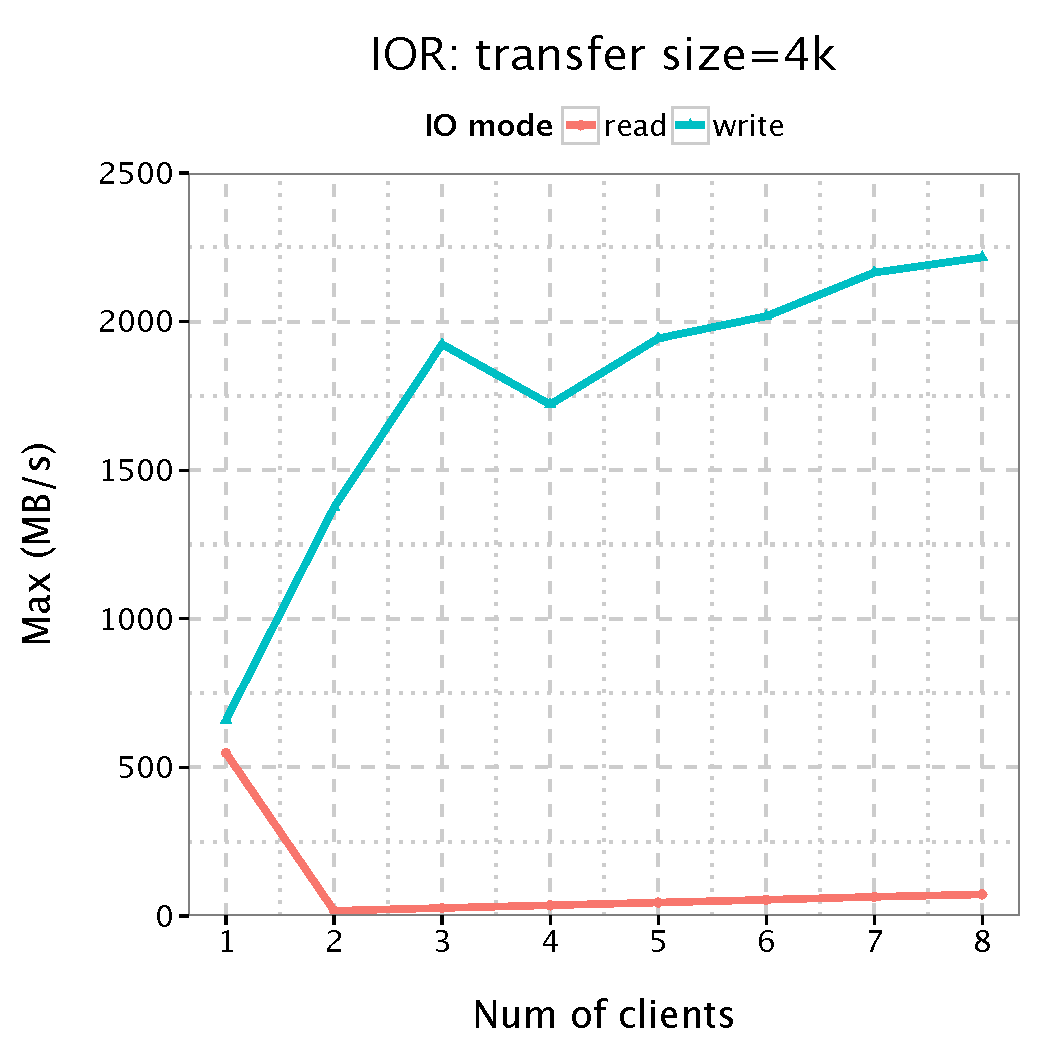
\includegraphics[width=3in]{data/ior_4k}
\caption{IOR tests: 4k transfer size}
\label{fig:ior4k}
\end{minipage}%
\begin{minipage}[t]{0.5\linewidth}
\centering
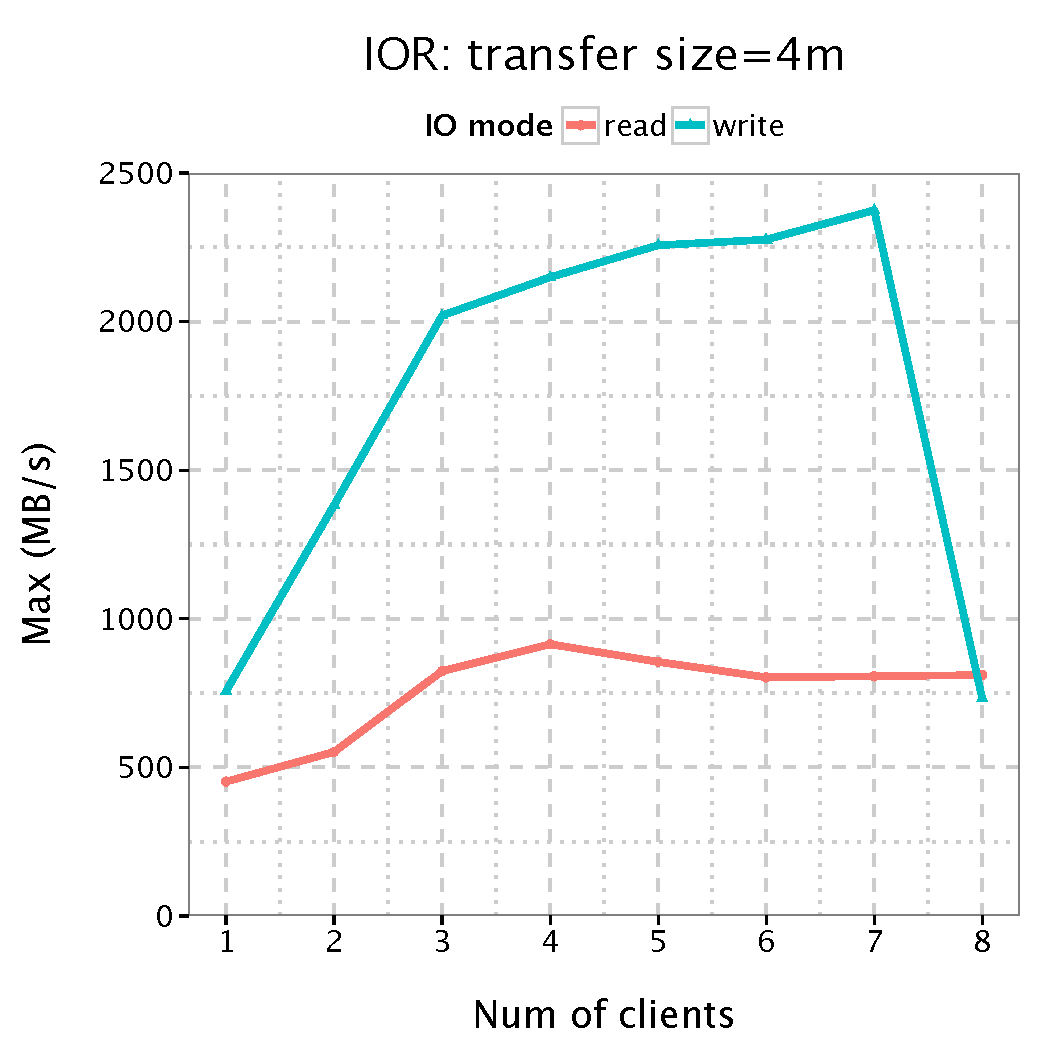
\includegraphics[width=3in]{data/ior_4m}
\caption{IOR tests: 4m transfer size}
\label{fig:ior4m}
\end{minipage}%
\end{figure}

Each client node has 6 GB physical memory, the block size is set so as to
mitigate the cache effect. In addition, the test harness program will issue the
following command at the beginning of each test: 
\begin{Verbatim}
# sync
# echo 3 | tee /proc/sys/vm/drop_caches
\end{Verbatim}



Here, 0 is the default value of \verb!drop_cahces!; 1 is to free pagecaches, 2
is to free dentries and inodes, 3 is to free pagecache, dentries, and inodes.



The full permutation of IOR parameters are not explored due to IO errors we ran
into (that is to be further investigated by the InkTank team). For the two
extreme cases we were to able to record, see Figure \ref{fig:ior4k} and
\ref{fig:ior4m}, we make the following observations:

\begin{itemize}
  \item The small read performance is almost an anomaly - we need to
  investigate why it is so low compare to write.
  \item The large read performance is almost half of the write performance,
  which is the opposite of RADOS level. 
  \item The write performance is cut in half compare to what we can obtain from
  RADOS benchmark. And number of clients reaches 8, there is a significant
  performance drop as well. 
\end{itemize}

\begin{figure}[htb]
\centering
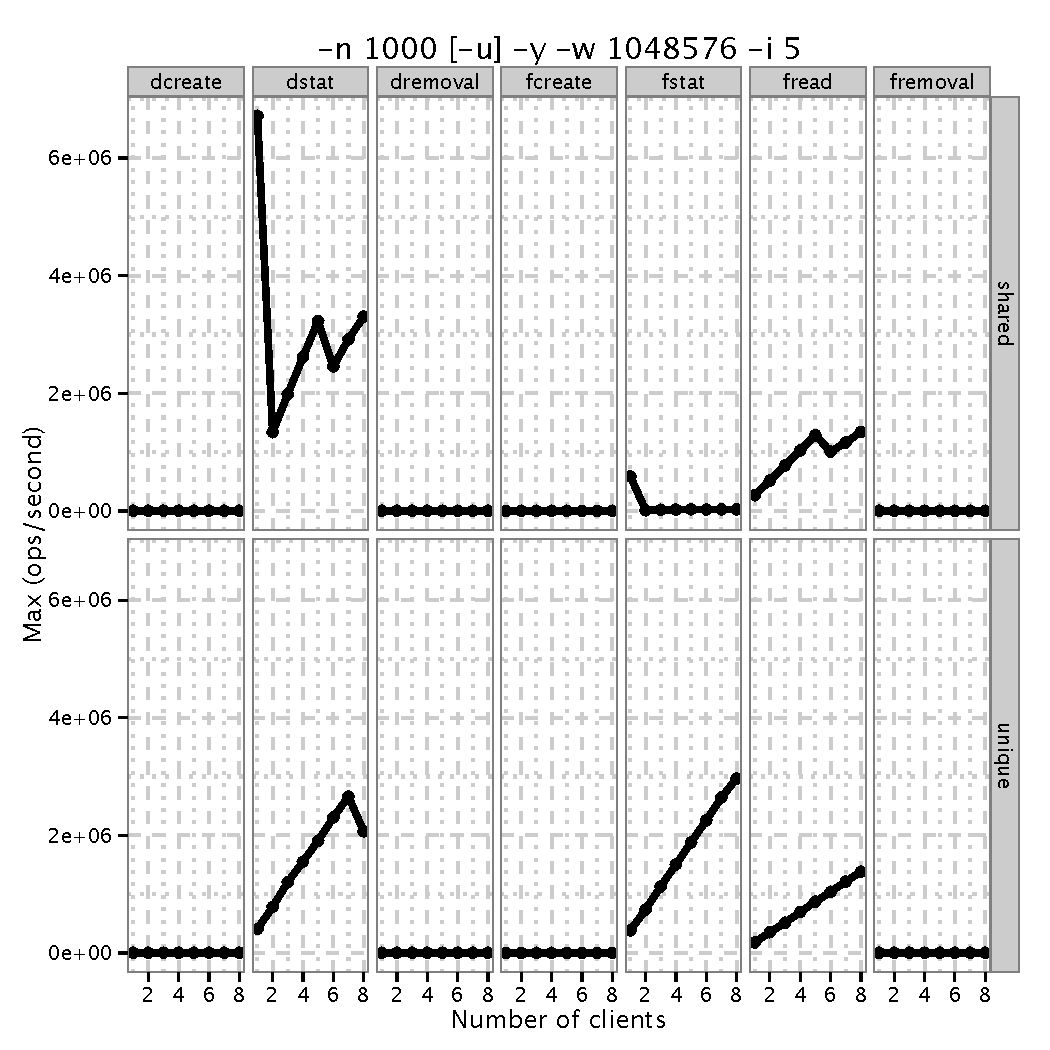
\includegraphics[width=5in]{data/mdtest}
\caption{mdtest of single MDS}
\label{fig:mdtest1c}
\end{figure}

\section{Metadata Performance}


In our particular setup, we have only one metadata server (MDS)
configured. Therefore, this is not a scalability test on the performance of
clustered MDS, which would be very interesting and might as well come later.
Instead, we focus on a single MDS, multiple clients (up to 8) and see how it
scales. The particular parameters we use for testing are:

\begin{itemize}
\item \verb!-w 1048576 -y!: for each created file, we write 1 MB data and
perform sync after it. This is a more realistic use case scenario than just
open, close and removal.

\item \verb!-n 1000!: this is per client file \textit{and} directories. For 8
clients, the number of files and directories is 8,000. Since we didn't specify
either \verb!-D! or \verb!-F!, so this is a mixture of both.

\item \verb!-d /mnt/cephfs/tmp!: we do specify a directory, but unlike under
Lustre file system, where you can have single client multiple mounts (for
increasing workload per client), here we just give the test an explicit home.

\item \verb!-u!: without this option, we are exercising shared directory; with
this option, we are exercising unique directories.

\end{itemize}

Each test iterates 5 times and we are showing the max. Figure
\ref{fig:mdtest1c} is meant to give an overview on the trending of each
directory (prefixed with d) and file (prefixed with f) operations, against the
number of clients. Due to the scale difference, it doesn't convey the
magnitude of lower numbers. We summarize the results as follows:

\begin{itemize}

\item Within a single sharing mode (either shared or unique directory), the
directory stat and file stat, as well as file read exhibit strong linear
scaling property. 

\item While the other operations seems unaffected or flat by the number of
clients, it is not so if we zoom in, see \ref{fig:mdtest-fcreate} and
\ref{fig:mdtest-dcreate}:  as number of clients increases, we observed the
contention for shared directory. The performance degradation amount to 50\% or
more.

\item Though the same saturation or degradation trend is not observed for file
creation, it is likely due to we have not put enough of workload stress on MDS.

\end{itemize}


\begin{figure}[htb]
\centering
%% -- 1st figure
\begin{minipage}[t]{0.5\linewidth}
\centering
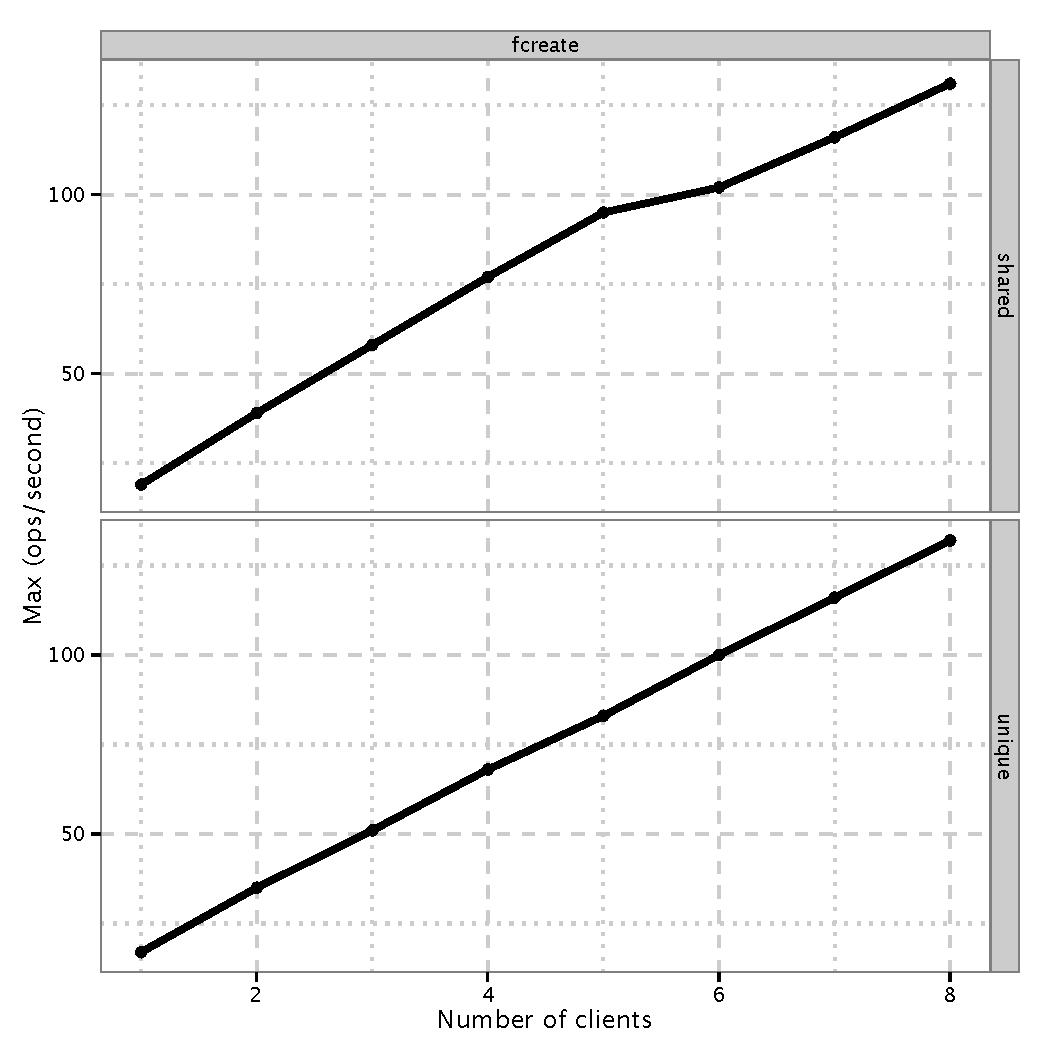
\includegraphics[width=3in]{data/mdtest-fcreate}
\caption{file creation vs.  \# of clients}
\label{fig:mdtest-fcreate}
\end{minipage}%
\begin{minipage}[t]{0.5\linewidth}
\centering
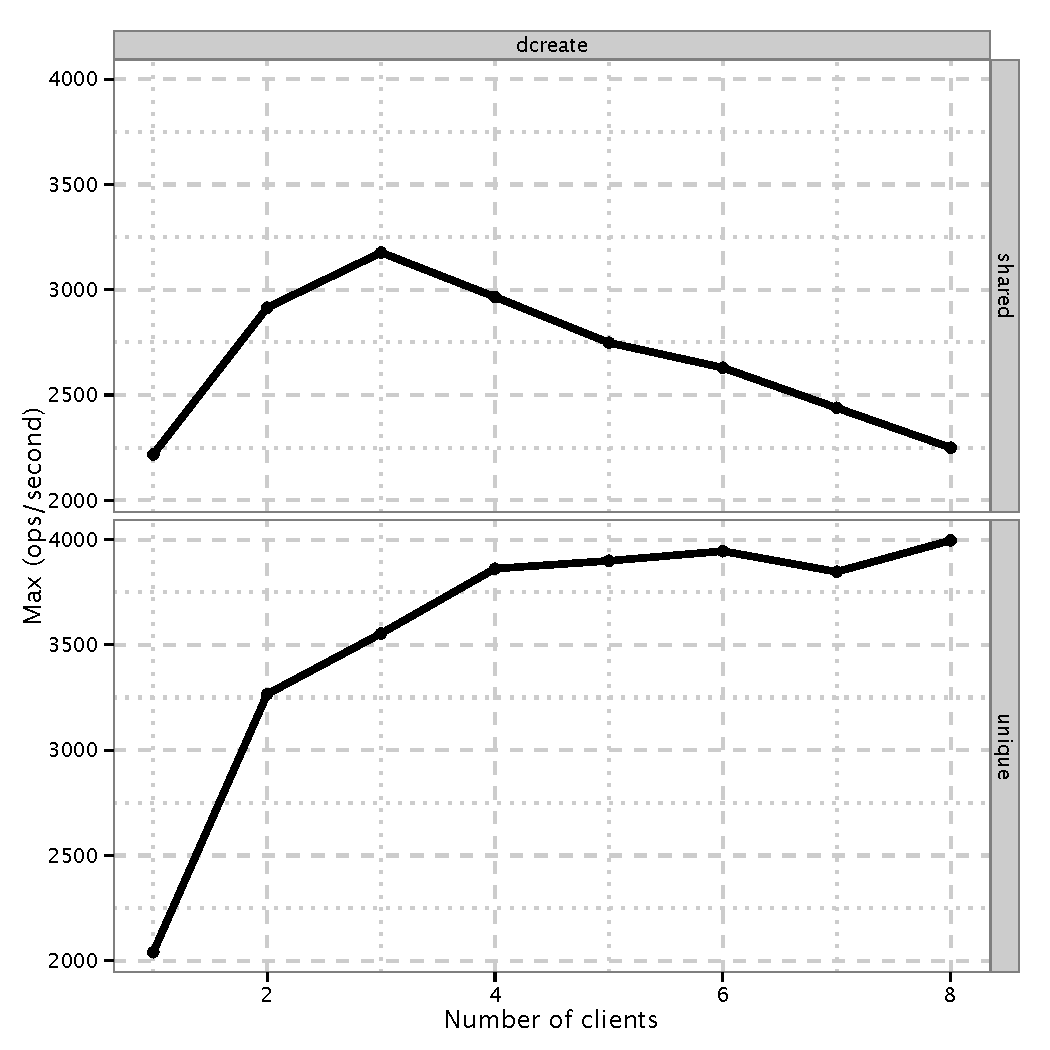
\includegraphics[width=3in]{data/mdtest-dcreate}
\caption{directory creation vs. \# of clients}
\label{fig:mdtest-dcreate}
\end{minipage}%
\end{figure}


\section{Observations and Conclusions}

This is preliminary observations from mostly performance perspective:

\begin{itemize}

  \item Ceph is built on the assumption that the underlying hardware components
  is unreliable, with little or no redundancy and failure detection capability.
  This is not the case in this leadership computing facilities. We have disabled
  replication for pools, but this will take a toll somewhere in the processing
  and we don't know if this is significant.

  \item Ceph do \textbf{metadata + data} journaling, which is fine for host
  system that has locally attached disk. However, this presents a problem in DDN
  SFA10-like hardware, where the backend LUNs are exposed as block device
  through SRP over IB. The journaling write would requires double bandwidth
  compare to Lustre-like metadata only journaling mechanism. For Ceph to anything
  viable in this facility, there has to be a solution for this.

  \item Ceph is observed to have consist results and linear scalability at the
  RADOS level. However, it broke down at the file system level with synthetic
  benchmark suite such as IOR. We have experience large performance swings
  during different runs, very low read performance when transfer size is small,
  and IO errors tend to happen when system is under stress (more clients and
  large transfer size). These are not particularly reproducible results, but it
  suggests the level of maturity still have a long way to go.
  
\end{itemize}

\section*{Appendix: CRUSH Map}

This crush map is just an example of full OSD mapping. As we create and
re-create different testbed with different OSD configurations, the map will
change accordingly.

\input{crush.txt}

\end{document}
